%%%%%%%%%%%%%%%%%%%%%%%%%%%%%%%%%%%%%%%%%%%%%%%%%%%%%%%%%%%%%%%%%%%%
%% I, the copyright holder of this work, release this work into the
%% public domain. This applies worldwide. In some countries this may
%% not be legally possible; if so: I grant anyone the right to use
%% this work for any purpose, without any conditions, unless such
%% conditions are required by law.
%%%%%%%%%%%%%%%%%%%%%%%%%%%%%%%%%%%%%%%%%%%%%%%%%%%%%%%%%%%%%%%%%%%%

\documentclass[
  digital, %% This option enables the default options for the
           %% digital version of a document. Replace with `printed`
           %% to enable the default options for the printed version
           %% of a document.
  twoside, %% This option enables double-sided typesetting. Use at
           %% least 120 g/m² paper to prevent show-through. Replace
           %% with `oneside` to use one-sided typesetting; use only
           %% if you don’t have access to a double-sided printer,
           %% or if one-sided typesetting is a formal requirement
           %% at your faculty.
  table,   %% This option causes the coloring of tables. Replace
           %% with `notable` to restore plain LaTeX tables.
  nolof,     %% This option prints the List of Figures. Replace with
           %% `nolof` to hide the List of Figures.
  nolot,     %% This option prints the List of Tables. Replace with
           %% `nolot` to hide the List of Tables.
  %% More options are listed in the user guide at
  %% <http://mirrors.ctan.org/macros/latex/contrib/fithesis/guide/mu/fi.pdf>.
]{fithesis3}
%% The following section sets up the locales used in the thesis.
\usepackage[resetfonts]{cmap} %% We need to load the T2A font encoding
%\usepackage[T1,T2A]{fontenc}  %% to use the Cyrillic fonts with Russian texts.
\usepackage[
  main=english, %% By using `czech` or `slovak` as the main locale
                %% instead of `english`, you can typeset the thesis
                %% in either Czech or Slovak, respectively.
  english, slovak, czech%german, russian, czech, slovak %% The additional keys allow
]{babel}        %% foreign texts to be typeset as follows:
%%
%%   \begin{otherlanguage}{german}  ... \end{otherlanguage}
%%   \begin{otherlanguage}{russian} ... \end{otherlanguage}
%%   \begin{otherlanguage}{czech}   ... \end{otherlanguage}
%%   \begin{otherlanguage}{slovak}  ... \end{otherlanguage}
%%
%% For non-Latin scripts, it may be necessary to load additional
%% fonts:
\usepackage{paratype}
\def\textrussian#1{{\usefont{T2A}{PTSerif-TLF}{m}{rm}#1}}
%%
%% The following section sets up the metadata of the thesis.
\thesissetup{
    date          = \the\year/\the\month/\the\day,
    university    = mu,
    faculty       = fi,
    type          = mgr,
    author        = Juraj S\'{i}\v{c},
    gender        = m,
    advisor       = {Jan Strej\v{c}ek},%\\ \textbf{Co-advisor:} Martin Jon\'{a}\v{s}},
    title         = {Satisfiability of DQBF Using Binary Decision Diagrams},
    TeXtitle      = {Satisfiability of DQBF Using Binary Decision Diagrams},
    keywords      = {dependency quantified Boolean formula, DQBF, binary decision diagram, BDD, satisfiability, solver},
    TeXkeywords   = {dependency quantified Boolean formula, DQBF, binary decision diagram, BDD, satisfiability, solver},
    abstract      = {%
      This is the abstract of my thesis, which can

      span multiple paragraphs.
    },
    thanks        = {%
      These are the acknowledgements for my thesis, which can

      span multiple paragraphs.
    },
    bib           = bibliography.bib
    %% Uncomment the following line (by removing the % symbol at
    %% the beginning) and replace `assignment.pdf` with the
    %% filename of your scanned thesis assignment.
    % assignment    = assignment.pdf,
}
\usepackage{makeidx}      %% The `makeidx` package contains
\makeindex                %% helper commands for index typesetting.
%% These additional packages are used within the document:
\usepackage{paralist} %% Compact list environments
\usepackage{amsmath}  %% Mathematics
\usepackage{amsthm}
\usepackage{amsfonts}
\usepackage{url}      %% Hyperlinks
\usepackage{tabularx} %% Tables
\usepackage{tabu}
\usepackage{booktabs}
\usepackage{listings} %% Source code highlighting
\lstset{
  basicstyle      = \ttfamily,
  identifierstyle = \color{black},
  keywordstyle    = \color{blue},
  keywordstyle    = {[2]\color{cyan}},
  keywordstyle    = {[3]\color{olive}},
  stringstyle     = \color{teal},
  commentstyle    = \itshape\color{magenta},
  breaklines      = true,
}
\usepackage{floatrow} %% Putting captions above tables
\floatsetup[table]{capposition=top}
%% The following code fixes the rendering of BibLaTeX ISO 690
%% references in old TeX Live (such as the one at Overleaf).
\thesisload
\makeatletter
\def\thesis@biblatexiso@fix@package{iso-numeric.bbx}
\def\thesis@biblatexiso@fix@end{\relax}
\newif\ifthesis@biblatexiso@fix@
\thesis@biblatexiso@fix@false
\def\thesis@biblatexiso@fix@next#1,{%
  \def\thesis@biblatexiso@fix@current{#1}%
  \ifx\thesis@biblatexiso@fix@current\thesis@biblatexiso@fix@package
    \thesis@biblatexiso@fix@true
  \fi
  \ifx\thesis@biblatexiso@fix@current\thesis@biblatexiso@fix@end
    \expandafter
    \@gobble
  \fi
  \thesis@biblatexiso@fix@next
}
\expandafter\expandafter\expandafter\thesis@biblatexiso@fix@next\@filelist,\relax,
\ifthesis@biblatexiso@fix@
  \defbibenvironment{bibliography}
    {\list%
       {\MethodFormat}%
       {\setlength{\labelwidth}{\labelnumberwidth}%
        \setlength{\leftmargin}{\labelwidth}%
        \setlength{\labelsep}{\biblabelsep}%
        \addtolength{\leftmargin}{\labelsep}%
        \setlength{\itemsep}{\bibitemsep}%
        \setlength{\parsep}{\bibparsep}}%
        \renewcommand*{\makelabel}[1]{\hss##1}
        }%
    {\endlist}%
  {\item}%
\fi
\makeatother

%%%%%%%%%%%%%%%%%%%%%%%%%%%%%%%%%%%%%%%%%%%%%%%%%%%%%%%%%
%%%%%%%%%%%%%%%%%%%%%%%%%%%%%%%%%%%%%%%%%%%%%%%%%%%%%%%%%
%%%%%% The packages I use, my definitions, etc. %%%%%%%%%
%%%%%%%%%%%%%%%%%%%%%%%%%%%%%%%%%%%%%%%%%%%%%%%%%%%%%%%%%
%%%%%%%%%%%%%%%%%%%%%%%%%%%%%%%%%%%%%%%%%%%%%%%%%%%%%%%%%

% for subfigures
\usepackage{subcaption}

% for writing nice pseudocode...
\usepackage{algpseudocode}
% ...and a float wrapper for them
\usepackage{algorithm}

\usepackage{mathtools}

% for checking for | in definition of set
\usepackage{xstring}

% for \set{}
\usepackage{braket}
% for notation { x | P(x)} we will use command \setbuilder
\let\setbuilder\set
% for {1,2,3}
\newcommand{\simpleset}[1]{\{{#1}\}}
% based on whether | is in the argument either use set builder notation or simple set notation
\renewcommand{\set}[1]{\normalexpandarg\IfSubStr{#1}{|}{\setbuilder{#1}}{\simpleset{#1}}}
%\renewcommand{\set}[1]{\simpleset{#1}}

% for semantic symbols [[ and ]]
\usepackage{stmaryrd}

% for nicer looking substitutions in formulas
\usepackage{nicefrac}

% for writing out rules of DQBF in NNF
\usepackage{ebproof}

% for complexity class
%\usepackage[basic]{complexity}

% for writing left aligned text in figures
%\usepackage{caption}

%% We will define several mathematical sectioning commands.
\newtheorem{theorem}{Theorem}[chapter] %% The numbering of theorems
                               %% will be reset after each chapter.
\newtheorem{lemma}[theorem]{Lemma}         %% The numbering of lemmas
\newtheorem{corollary}[theorem]{Corollary} %% and corollaries will
                               %% share the counter with theorems.
\theoremstyle{definition}
\newtheorem{definition}{Definition}
\newtheorem{example}{Example}
\theoremstyle{remark}
\newtheorem*{remark}{Remark}

% [[ #1 ]]
\newcommand{\seman}[1]{\left\llbracket {#1} \right\rrbracket}
% substitution for formulas: [phi'/phi] - \substitute{phi}{phi'}
\newcommand{\substitute}[2]{\left[ \nicefrac{#2}{#1} \right]}
% the set of all boolean formulas over #1
\newcommand{\BF}[1]{\mathbf{\Phi}_{#1}^{\normalfont{\text{\tiny BF}}}}
%\newcommand{\BF}[1]{BF(#1)}
% the set of all dependency quantified boolean formulas over #1
\newcommand{\DQBF}[1]{\mathbf{\Phi}_{#1}^{\normalfont{\text{\tiny DQBF}}}}
%\newcommand{\DQBF}[1]{\mathbf{\Phi}_{#1}^{\normalfont{\text{\tiny dnnf}}}}
% the set of all valuations over #1
\newcommand{\valtns}[1]{\mathbf{A}_{#1}}
% the set of all Boolean functions over #1
\newcommand{\BFuncs}[1]{\mathbb{F}_{#1}}

% the set of existential variables for formula #1
\newcommand{\evars}[1]{V_{#1}^{\exists}}
% the set of universal variables for formula #1
\newcommand{\uvars}[1]{V_{#1}^{\forall}}
% the set of free variables for formula #1
\newcommand{\fvars}[1]{V_{#1}^{\mathrm{free}}}
% the set of quantified variable for formula #1
\newcommand{\qvars}[1]{V_{#1}^{Q}}

% support set of boolean function #1
\newcommand{\supp}[1]{\mathrm{supp}(#1)}

% set of Skolem functions mapping for formula #1
\newcommand{\Scands}[1]{\mathbb{S}_{#1}}

% logical equality (like \lor or \land)
\newcommand{\lequal}{\Leftrightarrow}

% space between quantifiers and formula
\newcommand{\itholds}{\,}

% complexity classes
\newcommand{\ComplexityFont}[1]{%
{\ensuremath{\mathsf{#1}}}%extra {} makes everyone happy.
}
\newcommand{\PSPACE}{\ComplexityFont{PSPACE}}
\newcommand{\NP}{\ComplexityFont{NP}}
\newcommand{\NEXPTIME}{\ComplexityFont{NEXPTIME}}

%\renewcommand{\phi}{\varphi}

% for fixing overflowing in bibliography
\hyphenation{Chris-toph}
%\hyphenation{Mat-thias}

%%%%%%%%%%%%%%%%%%%%%%%%%%%%%%%%%%%%%%%%%%%%%%%%%%%%%%%%%
%%%%%%%%%%%%%%%%%%%%%%%%%%%%%%%%%%%%%%%%%%%%%%%%%%%%%%%%%

\begin{document}

\chapter{Introduction}

\chapter{Theory}
In this chapter we give the definitions and some theoretical results of dependency quantified Boolean formulas (DQBFs) and binary decision diagrams (BDDs). For DQBFs we build up from Boolean formulas (BFs) to which we add quantifiers resulting in quantified Boolean formulas (QBFs). After this, we add explicit dependencies to the definition of QBFs which results in DQBFs. For these we give two forms, one that can only have quantifiers at the beginning of the formula and one that allows them deeper in the formula. For the latter we give some rules for transformation of DQBFs which we use for developing our solver in Chapter~\ref{chap:algorithm}. 

In the last section of this chapter we define BDDs and recall some of their properties.

\section{Boolean Formulas}
We first start with defining Boolean formulas. For these we need a set of variables $V = \set{x_1, \dots, x_n}$ for which we can define a valuation function $v\colon V \to \{0,1\}$ that says whether each variable is true or false. We then define Boolean formulas as variables connected by logical operatives \emph{and} (${\land}$), \emph{or} (${\lor}$) and \emph{negation} (${\neg}$).

\begin{definition}
Let $V = \set{x_1, \dots, x_n}$ be a set of variables. The set of \emph{Boolean formulas} (BFs) \emph{over $V$}, denoted by $\BF{V}$, is defined as the smallest set fulfilling these conditions:
\begin{itemize}
    \item $0,1 \in \BF{V}$,
    \item $x \in \BF{V}$ if $x \in V$,
    \item $(\phi_1 \land \phi_2) \in \BF{V}$ if $\phi_1, \phi_2 \in \BF{V}$,
    \item $(\phi_1 \lor \phi_2) \in \BF{V}$ if $\phi_1, \phi_2 \in \BF{V}$,
    \item $\neg\phi \in \BF{V}$ if $\phi \in \BF{V}$.
\end{itemize}
\end{definition}
By $\phi\substitute{\phi_1}{\phi_2}$, where $\phi,\phi_1,\phi_2 \in \BF{V}$, we denote the BF $\phi$ where each occurrence of $\phi_1$ is replaced by $\phi_2$. We also use $(\phi_1 \lequal \phi_2)$ as a shorthand for the formula $((\phi_1 \land \phi_2) \lor (\neg \phi_1 \land \neg \phi_2))$.

A function $v\colon V \to \set{0,1}$ is called a \emph{valuation} over the set of variables $V$. A set of all valuations over $V$ is denoted by $\valtns{V}$. An \emph{evaluation} of $\phi \in \BF{V}$ in a valuation $v \in \valtns{V}$, denoted $v(\phi)$, is defined as %can extend this valuation to $\BF{V}$%, $v\colon \BF{V} \to \set{0,1}$ where
\begin{itemize}
    \item if $\phi = 0$ then $v(\phi) = 0$,
    \item if $\phi = 1$ then $v(\phi) = 1$,
    \item if $\phi = x_i$ where $x_i \in V$, then $v(\phi) = v(x_i)$,
    \item if $\phi = \neg\phi'$, then $v(\phi) = 1$ if $v(\phi') = 0$, otherwise $v(\phi) = 0$,
    \item if $\phi = (\phi_1 \land \phi_2)$, then $v(\phi) = 1$ if both $v(\phi_1) = 1$ and $v(\phi_2) = 1$, otherwise $v(\phi) = 0$, and
    \item if $\phi = (\phi_1 \lor \phi_2$), then $v(\phi) = 1$ if $v(\phi_1) = 1$ or $v(\phi_2) = 1$, otherwise $v(\phi) = 0$.
\end{itemize}
Each $\phi \in \BF{V}$ represents a \emph{Boolean function} $f_{\phi}\colon \valtns{V} \to \set{0,1}$ \emph{over $V$} such that $f_{\phi}(v) = v(\phi)$. Conversely, for each Boolean function we can find a BF representing it. The set of all Boolean functions over $V$ is denoted by $\BFuncs{V}$. The \emph{support set} $\supp{f}$ of Boolean function $f$ is defined as the set of variables occurring in a BF $\phi$ where $\phi$ represents $f$ and from all the BFs representing $f$, $\phi$ has the smallest number of variables occurring in it. That is, changing the values of variables that are not in the support set do not change the output value of $f$.


An important notion for BFs is \emph{satisfiability}. We say that $\phi \in \BF{V}$ is \emph{satisfiable} if there exists valuation $v \in \valtns{V}$ in which $\phi$ is true, that is $v(\phi) = 1$. Let $\phi_1, \phi_2 \in \BF{V}$. We say that they are \emph{equivalent}, denoted $\phi_1 \equiv \phi_2$, if for all valuations $v$ it holds that $v(\phi_1) = v(\phi_2)$. If they are either both satisfiable or they are both unsatisfiable, we call them \emph{equisatisfiable}, denoted $\phi_1 \approx \phi_2$.

\begin{example}
\label{ex:BF:prenex}
Let
\[\phi = ((x_1 \land x_2) \lequal (y_1 \lequal y_2)).\]
This formula says that if both $x_1$ and $x_2$ are true, then $y_1$ and $y_2$ must be same, otherwise they must be different. It is satisfiable, because in valuation $v$ such that $v(x_1) = v(x_2) = v(y_1) = v(y_2) = 1$ it holds that $\phi$ is evaluated to $v(\phi)=1$. The Boolean function $f_{\phi}$ that $\phi$ represents has support set $\supp{f_{\phi}} = \set{x_1, x_2, y_1, y_2}$.
%This formula is also equisatisfiable to formula 
%\[\phi' = (x \land y) \lor \neg x\] 
%because $\phi'$ is also satisfiable: in valuation $v'$ where $v'(x) = v'(y) = 1$ it holds that $v'(\phi') = 1$. Notice that even though $\phi$ and $\phi'$ have different variables, the equisatisfiability still holds. However, $\phi \not= \phi'$ because if we add to $v'$ that $v'(x_1) = v'(x_2) = v'(y_1) = 1$ and $v'(y_2) = 0$ we get that $v'(\phi) \not= v'(\phi')$.
\end{example}

\subsection{Conjuctive Normal Form}
\label{sec:BF:CNF}
To work with BFs it is usually easier to have them in some special form. The first one we define is called conjuctive normal form.

\begin{definition}
We say that boolean formula $\phi \in \BF{V}$ is in \emph{conjuctive normal form} (CNF) if there exist $\phi_1,\dots,\phi_n \in \BF{V}$ where
\[\phi = \phi_1 \land \dots \land \phi_n\]
and
\[\phi_i = l_{i1} \lor \dots \lor l_{i{m_i}}\]
for each $i = 1, \dots, n$, and for each $l_{ij}$ where $j \in \set{1,\dots,m_i}$ either $l_{ij} = x$ or $l_{ij} = \neg x$ for some $x \in V$.
\end{definition}
Formulas $\phi_1,\dots,\phi_n$ are called clauses and $l_{ij}$ are called literals. That is BF is in CNF if it is a conjuction of clauses which are disjunctions of literals, where literal is either a variable or its negation.

\begin{example}
The formula
\[\phi_{CNF} = (x \lor \neg y) \land (\neg x \lor y)\]
is in CNF with clauses $(x \lor \neg y)$ and $(\neg x \lor y)$ and literals $x,\neg y, \neg x$ and $y$.
\end{example}

For every BF $\phi$ there exists an equivalent formula in CNF which can be exponentially larger than $\phi$. However, by using Tseytin transformation~\cite{Tseitin} we can create an equisatisfiable BF $\phi_{CNF}$ which is only polynomially larger than the original BF $\phi$.

\subsection{Negation Normal Form}
\label{sec:BF:NNF}
We say that BF $\phi$ is in negation normal form (NNF) if negation occurs only in front of the variable. Each BF $\phi$ can be easily transformed into an equivalent BF $\phi'$ in NNF by applying these three rules:
\begin{enumerate}
    \item $\neg(\phi_1 \land \phi_2) \equiv (\neg\phi_1 \lor \neg\phi_2)$ 
    \item $\neg(\phi_1 \lor \phi_2) \equiv (\neg\phi_1 \land \neg\phi_2)$
    \item $\neg\neg x \equiv x$
\end{enumerate}
\begin{example}
Formula $\neg (x_1 \land (x_2 \lor \neg x_3))$ that is not in NNF is by using the first rule equal to $(\neg x_1 \lor \neg(x_2 \lor \neg x_3))$ which is by using the second rule equal to $(\neg x_1 \lor (\neg x_2 \land \neg\neg x_3))$. Finally, by using the third rule we get $(\neg x_1 \lor (\neg x_2 \land x_3))$ which is in NNF.
\end{example}

\section{Quantified Boolean Formulas}
Having defined BFs, we can move to the next step on the way to defining DQBF by adding quantifiers. We add existential (${\exists}$) and universal (${\forall}$) quantifiers bounded to variables which results in the definition of \emph{quantified Boolean formulas} (QBFs). Usually, definitions of QBFs allow quantifiers everywhere inside formula but we only give definition of one special form of QBFs called prenex normal form. In this form, QBFs allow quantifiers only at the beginning of the formula. However, this does not change the expressibility as it is possible to transform every QBF into prenex normal form~\cite{prenexingQBFs}.

%TODO: zmazat coloneqq a asi len nahradit s =
\begin{definition}
Let $V = \set{x_1,\dots,x_n}$ be a set of variables and $\phi \in \BF{V}$. A \emph{quantified Boolean formula} (QBF) $\psi$ over $V$ in closed prenex form is given by
\[\psi \coloneqq Q_1 x_1 Q_2 x_2 \dots Q_n x_n \itholds \phi\]
where $x_i \in V$ are distinct for all $i \in \set{1,2,\dots,n}$ and $Q_i \in \set{{\exists}, {\forall}}$.
\label{def:QBF}
\end{definition}

The BF $\phi$ is called the \emph{matrix} of $\psi$ and $Q_1 x_1 Q_2 x_2 \dots Q_n x_n$ is called the \emph{quantifier prefix} of $\psi$. A variable $x_i$ is called \emph{existential} if $Q_i = \exists$ and \emph{universal} if $Q_i = \forall$. The set of all existential variables of QBF $\psi$ is denoted by $\evars{\psi}$ and the set of all universal variables of $\psi$ is denoted by $\uvars{\psi}$. We define a level function $l\colon V \to \mathbb{N}$ which maps to each variable the number of quantifiers occurring before the variable in the formula. That is the variable $x_i \in V$ from QBF $\psi$ of Definition~\ref{def:QBF} has level $l(x_i) = i$. We denote the set of variables with level less than some $n \in \mathbb{N}$ as $V_{\psi}^{<n} = \set{x \in V | l(x) < n}$.

Again, we define satisfiability. Usually, satisfiability for QBFs is defined trough valuation function as in BFs case where evaluation of QBFs follows the same rules as BFs with two newly added rules for quantifiers:
\begin{itemize}
    \item $v(\forall x Q_i x_i \dots Q_n x_n \itholds \phi) = 1$ if both $v(Q_i x_i \dots Q_n x_n \itholds \phi\substitute{x}{0}) = 1$ and $v(Q_i x_i \dots Q_n x_n \itholds \phi\substitute{x}{1}) = 1$, otherwise it equals $0$,
    %TODO: check if the linebreak is not obvious
    \item $v(\exists x Q_i x_i \dots Q_n x_n \itholds \phi) = 1$ if $v(Q_i x_i \dots Q_n x_n \itholds \phi\substitute{x}{0}) = 1$ or \\ $v(Q_i x_i \dots Q_n x_n \itholds \phi\substitute{x}{1}) = 1$, otherwise it equals $0$.
\end{itemize}
We follow different but equal definition based on Skolemization, which replaces each existential variable $x$ by some Boolean function over universal variables with lower level than $x$. This is better suited to show a correspondence of QBFs and DQBFs when we add dependencies in the next section. A QBF $\psi$ of Definition~\ref{def:QBF} is satisfiable if for each $x \in V_{\psi}^{\exists}$ there exists a function $s_{x} \in \BFuncs{\uvars{\psi}\cap V_{\psi}^{<l(x)}}$ (called \emph{Skolem function}) such that the matrix $\phi$ of $\psi$, where every $x \in \evars{\psi}$ is replaced by some BF that represents $s_x$, is evaluated to $1$ in every valuation $v\colon \uvars{\psi} \to \set{0,1}$.

\begin{example}
\label{ex:QBF:prenex}
Let 
\[\psi = \forall x_1 \forall x_2 \exists y_1  \exists y_2 \itholds ((x_1 \land x_2) \lequal (y_1 \lequal y_2))\]
be a QBF where the matrix is formula $\phi$ from Example~\ref{ex:BF:prenex}. This QBF is satisfiable because for all values of $x_1, x_2$ we can find values of $y_1$ and $y_2$ such that they are same if $x_1 = x_2 = 1$ and different otherwise. The Skolem functions for this formula are for example $s_{y_1}$ which is represented by BF $x_1 \land x_2$ and $s_{y_2}$ which is represented by BF $1$. If we replace existential variables with their Skolem functions we get BF
\[((x_1 \land x_2) \lequal ((x_1 \land x_2) \lequal 1))\]
which is true in all valuations.
\end{example}

\section{Dependency Quantified Boolean Formulas}
Quantifiers have expanded the succinctness of BFs quite considerably. However, there is still one drawback of QBFs --- quantified variable $x$ depends on all variables that are quantified before $x$ in the formula. The question arises whether it is possible to give a definition of formula where the dependency relation is somehow explicitly given. The answer is yes, we can use \emph{dependency quantified Boolean formulas} (DQBFs).

DQBFs allow existential variables to be non-linearly dependent on the set of universal variables by explicitly writing out the set of universal variables on which each existential variable is dependent. The universal variables from this set are then used as the support set of the Skolem function of the existential variable which allows for even greater succinctness of DQBFs over QBFs.  

We start with the definition of DQBFs in prenex normal form on which we explain the basic notions and then we give the definition of DQBFs in non-prenex negation normal form which allows quantifiers inside formulas. Following this, we give theorems that show which DQBFs are equisatisfiable and can be replaced with each other thus allowing us to eliminate or push quantifiers inside the formula.
%\begin{itemize}
%    \item pushing quantifiers inside formula,
%    \item elimination of quantified variables or
%    \item ????removal of universal variables from the dependency sets of existential variables.????
%\end{itemize}

\subsection{Prenex Normal Form}
The first definition of DQBF form called prenex normal form is an analogy of the prenex normal form of QBFs.


%definicia DQBF -ak robim nonprenex tak zacat s prenex ale vysvetlit ze pre jednoduchost zacneme s tym + semantika prenex + priklady
\begin{definition}
  Let $V = \set{x_1, \dots, x_n, y_1, \dots, y_m}$ be a set of variables and $\phi \in \BF{V}$ a BF over $V$. A \emph{dependency quantified Boolean formula} (DQBF) $\psi$ in \emph{prenex normal form} (PNF) is given by
  \[\psi \coloneqq \forall x_1 \dots \forall x_n \exists y_1 (D_1) \dots \exists y_m (D_m) \itholds \phi\]
  where $D_i \subseteq \set{x_1, \dots, x_n}$ for each $i \in \set{1,\dots,m}$ is a \emph{dependency set} of variable $y_i$.
  \label{def:DQBF:PNF}
\end{definition}
We call the BF $\phi$ the \emph{matrix} of $\psi$ and $\forall x_1 \dots \forall x_n \exists y_1 (D_1) \dots \exists y_m (D_m)$ the \emph{quantifier prefix} of $\psi$. We call the variables from $\evars{\psi} = \set{y_1,\dots,y_m}$ \emph{existential} and variables from $\uvars{\psi} = \set{x_1,\dots,x_n}$ \emph{universal}. We also say that $\psi$ is in \emph{prenex conjuctive normal form} (PCNF) if it is in PNF where the matrix is in CNF.



\begin{example}
Let us use an example by Rabe~\cite{DQBFProofSystem} to explain the meaning behind dependency sets. Let 
\[\psi = \forall x_1 \forall x_2 \exists y_1 (x_1) \exists y_2 (x_2) \itholds ((x_1 \land x_2) \lequal (y_1 \lequal y_2))\]
be a DQBF. The matrix is the BF $\phi$ from Example~\ref{ex:BF:prenex} and the quantifier prefix is very similar to the QBF from Example~\ref{ex:QBF:prenex} but now both $y_1$ and $y_2$ depend only on one variable, $x_1$ and $x_2$ respectively. The QBF was satisfiable but this DQBF is not. To show why, we can look at it as a game where $y_1$  and $y_2$ are trying to satisfy the formula and $x_1,x_2$ are trying to make it false. However, $y_1$ knows only how $x_1$ is behaving and similarly $y_2$ knows only what $x_2$ is doing. As explained in Example~\ref{ex:BF:prenex} the matrix says that if both $x_1$ and $x_2$ are true, then $y_1$ and $y_2$ should be same, otherwise they need to be different. However, this is not possible, because if for example both $y_1,y_2$ decide to be true (similarly for false) when their respective universal variables are true then if one of the universal variable change, for example $x_1$ turns to false, then $y_2$ does not know about this and stays true. In that case $y_1$ has to change the value to false so they become different. The same thing happens to $y_2$ if $x_2$ changes its value to false. So we get behaviour where both existential variables just copy the behaviour of their universal variable. But at the end, if both $x_1$ and $x_2$ change their values to false, then the values of $y_1$ and $y_2$ are the same (false) which makes the formula $\psi$ false.
\end{example}

With the example in mind, we define satisfiability for DQBF in PNF similarly to how satisfiability is defined for QBFs with Skolem functions. DQBF $\psi$ of Definition~\ref{def:DQBF:PNF} is \emph{satisfiable} if for each $y \in \evars{\psi}$ there exists a Skolem function $s_y \in \BFuncs{D_y}$ such that $\phi$, where each $y \in \evars{\psi}$ is replaced by a BF representing Boolean function $s_y$, evaluates to $1$ in all valuations $v\colon \uvars{\psi} \to \set{0,1}$.

\begin{example}
The possible Skolem functions $s_{y_1}$ for existential variable $y_1$ from the previous example are those that are represented by BFs $0$, $1$, $x_1$ or $\neg x_1$. For $y_2$ the Skolem functions $s_{y_2}$ can be those that are represented by BFs $0$, $1$, $x_2$ or $\neg x_2$. However, we cannot choose a pair $s_{y_1}$ and $s_{y_2}$ such that by replacing $y_1$ and $y_2$ with them, we get a BF that is true in all valuations. In the previous example we actually used $s_{y_1}$ represented by $x_1$ and $s_{y_2}$ represented by $x_2$, where we get BF
\[((x_1 \land x_2) \lequal (x_1 \lequal x_2))\]
which is obviously not true in all valuations.
\end{example}

\begin{remark}
QBFs in PNF can be seen as a special case of DQBFs in PNF where the dependency sets are linearly ordered. That is a DQBF $\psi$ where for each two dependency sets $D_{y_1}$ and $D_{y_2}$ it holds that either $D_{y_1} \subseteq D_{y_2}$ or $D_{y_2} \subseteq D_{y_1}$, can be easily transformed to QBF by reordering the quantifiers.
\end{remark}

\subsection{Negation Normal Form}
In this section we give the definition of the normal form of DQBF that is non-prenex. This allows quantifiers inside the formula. However, negation is only allowed in front of variables. %This restriction stems from the fact that prenex DQBFs are not syntactically closed under negation~\cite{NegationOfDQBFs}. %, therefore negation in front of some quantified subformula would make no sense.
This form is also not closed which means it allows free variables. These variables are not bounded by any quantifier thus the definition of satisfiability has to take them into consideration. The definitions in this section are taken from Ge-Ernst et al.~\cite{HQSquantifierLocalization}.


We first give the definition of the set $\DQBF{V}$ of DQBFs in \emph{negation normal form} where we use the rules form Figure~\ref{fig:DQBFrules}. Each rule has the list of conditions (over the line) that has to hold so that the resulting formula under the line is in $\DQBF{V}$. For each formula $\psi$ we also define the set of existential $\evars{\psi}$, universal $\uvars{\psi}$, and free $\fvars{\psi}$ variables. We also use $\qvars{\psi} = \evars{\psi} \cup \uvars{\psi}$ and $V_{\psi} = \qvars{\psi} \cup \fvars{\psi}$.  Furthermore, $\psi^{-v}$ result from $\psi$ where $v$ is removed from every dependency set in $\psi$. 

\begin{figure}[htp]
    \renewcommand{\arraystretch}{2}
    %\begin{centering}
    %\hspace*{-0.7cm}
    \begin{tabular}{ccccc}
        \multicolumn{2}{c}{rule} & $V_{.}^{\exists}$ & $V_{.}^{\forall}$ & $V_{.}^{\text{free}}$\\\hline
        {\begin{prooftree}
            \infer0{0 \in \DQBF{V}}
        \end{prooftree}}
        & {\begin{prooftree}
            \infer0{1 \in \DQBF{V}}
        \end{prooftree}}
        & $\emptyset$ & $\emptyset$ & $\emptyset$\\[5mm]
        {\begin{prooftree}
            \hypo{v \in V}
            \infer1{v \in \DQBF{V}}
        \end{prooftree}}
        %& $\emptyset$ & $\emptyset$ & $\set{v}$\\[5mm]
        & {\begin{prooftree}
            \hypo{v \in V}
            \infer1{\neg v \in \DQBF{V}}
        \end{prooftree}}
        & $\emptyset$ & $\emptyset$ & $\set{v}$\\[5mm]
        \multicolumn{2}{c}{{\begin{prooftree}
            \hypo{\psi_1 \in \DQBF{V}}
            \hypo{\psi_2 \in \DQBF{V}}
            \hypo{(\ref{disconjrule})}
            \infer3{(\psi_1 \land \psi_2) \in \DQBF{V}}
        \end{prooftree}}}
        & $\evars{\psi_1} \cup \evars{\psi_2}$ & $\uvars{\psi_1} \cup \uvars{\psi_2}$ & $\fvars{\psi_1} \cup \fvars{\psi_2}$\\[5mm] 
        \multicolumn{2}{c}{{\begin{prooftree}
            \hypo{\psi_1 \in \DQBF{V}}
            \hypo{\psi_2 \in \DQBF{V}}
            \hypo{(\ref{disconjrule})}
            \infer3{(\psi_1 \lor \psi_2) \in \DQBF{V}}
        \end{prooftree}}}
        & $\evars{\psi_1} \cup \evars{\psi_2}$ & $\uvars{\psi_2} \cup \uvars{\psi_2}$ & $\fvars{\psi_1} \cup \fvars{\psi_2}$\\[5mm]
        \multicolumn{2}{c}{{\begin{prooftree}
            \hypo{\psi \in \DQBF{V}}
            \hypo{v \in V \setminus \qvars{\psi}}
            \hypo{(\ref{existrule})}
            \infer3{\exists v(D_v)\itholds\psi^{-v} \in \DQBF{V}}
        \end{prooftree}}}
        & $\evars{\psi} \cup \set{v}$ & $\uvars{\psi}$ & $\fvars{\psi} \setminus \set{v}$ \\[5mm]
        \multicolumn{2}{c}{{\begin{prooftree}
            \hypo{\psi \in \DQBF{V}}
            \hypo{v \in V \setminus \qvars{\psi}}
            \infer2{\forall v\itholds\psi \in \DQBF{V}}
        \end{prooftree}}}
        & $\evars{\psi}$ & $\uvars{\psi} \cup \set{v}$ & $\fvars{\psi} \setminus \set{v}$\\[5mm]
    \end{tabular}
    %\end{centering}
    \flushleft{where (\ref{disconjrule}) refers to}
    \begin{multline}
        \tag{1} \label{disconjrule}
        \qvars{\psi_1} \cap \qvars{\psi_2} = \emptyset \text{\quad and\quad} \fvars{\psi_1} \cap \qvars{\psi_2} = \emptyset \text{\quad and\quad} \fvars{\psi_2} \cap \qvars{\psi_1} = \emptyset
    \end{multline}
    \flushleft{and (\ref{existrule}) refers to}
    \begin{equation}
        \tag{2} \label{existrule}
        D_v \subseteq V \setminus (\qvars{\psi} \cup \set{v})
    \end{equation}
    \caption{Rules defining the syntax of DQBFs in NNF (based on Ge-Ernst et al.~\cite{HQSquantifierLocalization}).}
    \label{fig:DQBFrules}
\end{figure}

\begin{definition}
  Let $V$ be a set of variables. The set $\DQBF{V}$ of \emph{DQBFs in negation normal form} (NNF) over $V$ is defined to be the smallest set satisfying the rules from Figure~\ref{fig:DQBFrules}.
\end{definition}
\begin{remark}
In the definition by Ge-Ernst et al.~\cite{HQSquantifierLocalization} the last two rules in Figure~\ref{fig:DQBFrules} have condition $v \in \fvars{\psi}$ instead of $v \in V \setminus \qvars{V}$. This condition is too strong and does not allow some formulas which are valid. For example, as we show in the next section, we can transform DQBFs by pushing quantifiers inside the formula and this way we can end up with a formula $\forall x \itholds \psi$ where $x \not\in V_{\psi}$. However, according to the definition by Ge-Ernst et al.~\cite{HQSquantifierLocalization} this would not be a valid formula.
\end{remark}

\begin{remark}
Notice that each DQBF $\psi$ in PNF can be transformed into DQBF $\psi'$ in NNF by transforming the matrix of $\psi$ to NNF as explained in Section~\ref{sec:BF:NNF}.
\end{remark}

By $\psi\substitute{x_1}{x_2}$ where $\psi \in \DQBF{V}$, $x_1, x_2 \in V$, $x_2 \not\in V_{\psi}$ we denote the DQBF $\psi$ in which every occurence of $x_1$ (even in the dependency sets) is replaced by $x_2$. If $x_1 \not\in \qvars{\psi}$ and is not in any dependency set in $\psi$ then by $\psi\substitute{x_1}{\kappa}$, where $\kappa\in\set{0,1}$, we denote the DQBF $\psi$ in which every occurence of $x_1$ is replaced by $\kappa$.

% semantics
The definition of satisfiability of DQBF in NNF follows the same way as in the previous section but now we have to decide what to do with free variables. In non-prenex case of QBFs, free variables are usually assumed to be existential variables with quantifiers at the beginning of the formula. In DQBF case this means that free variables would have empty dependency sets so the definition needs to follow that. We first define mapping, called \emph{Skolem functions mapping} which maps to each existential and free variables some Skolem function fulfilling conditions set by dependency sets. Then we define \emph{semantics} of DQBFs in NNF as the set of Skolem functions mappings which satisfy the formula.

\begin{definition}[Skolem Functions Mapping]
  Let $\psi \in \DQBF{V}$. We say that mapping $s\colon (\evars{\psi} \cup \fvars{\psi}) \to \BFuncs{\uvars{\psi}}$ is a \emph{Skolem functions mapping} of $\psi$ if
  \begin{itemize}
      \item $\supp{s(v)} \subseteq (D_v \cap \uvars{\psi})$ for all $v \in \evars{\psi}$ and
      \item $\supp{s(v)} = \emptyset$ for all $v \in \fvars{\psi}$, i.e. $s(v)$ is either represented by $0$ or $1$.
  \end{itemize}
\end{definition}

The set of all Skolem functions mappings of $\psi$ is denoted by $\Scands{\psi}$. If $s \in \Scands{\psi}$, we write $s(\psi)$ for the formula that results from $\psi$ by replacing each existential and free variable $v$ by a BF that represents $s(v)$ and omitting all quantifiers from $\psi$. This results in a BF containing only variables from $\uvars{\psi}$.

\begin{definition}[Semantics]
  Let $\psi \in \DQBF{V}$. We define the \emph{semantics} $\seman{\psi}$ of $\psi$ as follows:
  \[\seman{\psi} = \set{s \in \Scands{\psi} | v(s(\psi))=1 \text{ for all } v \in \valtns{\uvars{\psi}}}.\]
\end{definition}
Formula $\psi$ is \emph{satisfiable} iff $\seman{\psi} \not= \emptyset$ and the elements of $\seman{\psi}$ are \emph{satisfiying} Skolem functions mappings of $\psi$. We say that two formulas $\psi_1$ and $\psi_2$ are \emph{equisatisfiable}, denoted $\psi_1 \approx \psi_2$, if both are either satisfiable or both are unsatisfiable.
\begin{example}
\label{ex:DQBF:NNF}
To explain the semantics of DQBF in NNF we use the example by Ge-Ernst et al.~\cite{HQSquantifierLocalization}:
\[\psi = \forall x_1 \forall x_2\itholds ((x_1 \lequal x_2) \lor \exists y (x_2)\itholds \neg(x_1 \lequal y)).\]
The meaning behind this formula is that either $x_1$ and $x_2$ are the same or there is some $y$ which is dependent only on $x_2$ which is different from $x_1$. The Skolem functions mappings of $\psi$ are then $\Scands{\psi} = \{y\mapsto f_0$, $y\mapsto f_1$, $y\mapsto f_{x_2}$, $y\mapsto f_{\neg x_2}\}$ where $f_0$ is the Boolean function represented by Boolean formula $0$, $f_1$ is represented by $1$, $f_{x_2}$ by $x_2$ and $f_{\neg x_2}$ by $\neg x_2$. It is obvious that only $s = y \mapsto f_{x_2}$ is a satisfying mapping of $\psi$, since only $s(\psi) = ((x_1 \lequal x_2) \lor \neg(x_1 \lequal x_2))$ is true in all valuations.
\end{example}

\subsection{Localising Quantifiers}
\label{sec:quantLocalization}
Now that we have defined DQBFs we give some theoretical results which show the equisatisfiability of different DQBFs which can result in their simplification. These results can be then used for developing a DQBF solver which checks whether an input DQBF is satisfiable or not.

We start with two theorems that show when it is possible to push (extract) quantifiers in (from) the formula. %The first theorem is from~\cite[Theorem 3]{HQSquantifierLocalization} where ... is replaced by ... from~\cite[Theorem 4]{HQSquantifierLocalization}

\begin{theorem}[{\cite[Theorems 3,4]{HQSquantifierLocalization}}]
\label{thrm:quantLocalEq}
  Let ${\diamond} \in \set{{\land},{\lor}}$ and $\psi,\psi_1,\psi_2 \in \DQBF{V}$. We assume that $x'$ and $y'$ are fresh variables, which do not occur in $\psi,\psi_1$ and $\psi_2$. The following equisatifiabilities hold for all DQBFs in NNF:
  \begin{align}
      %\forall x : \psi &\approx \psi \text{, if } x \not\in V_{\psi} \\
      \forall x \itholds (\psi_1 \land \psi_2) &\approx (\forall x \itholds \psi_1) \land (\forall x' \itholds \psi_2\substitute{x}{x'}) \label{loc:unconj1} \\
      \forall x \itholds (\psi_1 \land \psi_2) &\approx (\psi_1^{-x} \land (\forall x \itholds \psi_2)) \text{, if } x \not\in V_{\psi_1} \label{loc:unconj2} \\
      \forall x \itholds (\psi_1 \lor \psi_2) &\approx \begin{multlined}[t][3cm](\psi_1 \lor (\forall x \itholds \psi_2)) \text{, if } x \not\in V_{\psi_1} \label{loc:undisj} \\
      \text{ and } x \not\in D_y \text{ for all } y \in \evars{\psi_1}\end{multlined} \\
      \exists y(D_y) \itholds (\psi_1 \lor \psi_2) &\approx (\exists y(D_y) \itholds \psi_1) \lor (\exists y'(D_y) \itholds \psi_2\substitute{y}{y'}) \label{loc:exdisj} \\
      \exists y(D_y) \itholds (\psi_1 \diamond \psi_2) &\approx (\psi_1 \diamond (\exists y(D_y) \itholds \psi_2)) \text{, if } y \not\in V_{\psi_1} \label{loc:exboth} \\
      \exists y_1(D_{y_1})\exists y_2(D_{y_2}) \itholds \psi &\approx \exists y_2(D_{y_2}) \exists y_1(D_{y_1}) \itholds \psi \label{loc:exswap} \\
      \forall x_1\forall x_2 \itholds \psi &\approx \forall x_2\forall x_1 \itholds \psi \label{loc:unswap} \\
      \forall x\exists y(D_y) \itholds \psi &\approx \exists y(D_y)\forall x \itholds \psi\text{, if } x \not\in D_y. \label{loc:bothswap}
  \end{align}
\end{theorem}

The next theorem shows that if DQBFs from the previous theorem occur as subformulas of DQBF $\psi$ they can be replaced without changing the satisfiability of $\psi$.

\begin{theorem}
  Let $\psi \in \DQBF{V}$, $\phi_1$ be the left side formula and $\phi_2$ be the right side formula  from the same equality from Theorem~\ref{thrm:quantLocalEq} where $\phi_1$ is a subformula of $\psi$. Again, the same assumptions for $x'$ and $y'$ variables hold as in Theorem~\ref{thrm:quantLocalEq} but also they do not occur in $\psi$. Then $\psi \approx \psi'$ where $\psi'$ results from $\psi$ by replacing $\phi_1$ with $\phi_2$.
\end{theorem}
\begin{proof}
  (\ref{loc:unconj1}) We show that $\seman{\psi} \not= \emptyset$ iff $\seman{\psi'} \not= \emptyset$. First, let $s \in \seman{\psi}$. We now show that for $s'$, where $s'(y) = s(y)\substitute{x}{x'}$ for $y \in \evars{\phi_2}$ and $s'(y) = s(y)$ otherwise, it holds $s' \in \seman{\psi'}$. Let $v \in \valtns{\psi'}$. We need to show that $v(s'(\psi')) = 1$. Because $s \in \seman{\psi}$ it holds that $v(s(\psi)) = 1$. For the case that $v(x') = v(x)$ we get $v(s(\psi)) = v(s'(\psi'))$, because BFs $s(\psi)$ and $s(\psi')$ differ only in some replacements of $x$ by $x'$. Therefore we assume that $v(x') \not= v(x)$. We know that $\psi$ and $\psi'$ differ only in the formulas $\phi_1$ and $\phi_2$, therefore we can only focus on the case that $v(s(\psi))$ depends on the value of $v(s(\phi_1))$. Also, $\psi$ is in NNF, which means that in the tree of operations, negation cannot be before $\phi_1$. This means that we can focus only on the case where $v(s(\phi_1)) = 1$, otherwise the value of $v(s(\psi))$ would not depend on $v(s(\phi_1))$. This means we need to show that $v(s'(\phi_2)) = 1$. We have that for $v(s(\phi_1)) = v(s(\forall x \itholds (\psi_1 \land \psi_2))) = v(s(\psi_1) \land s(\psi_2))$ to be equal to one, it has to hold that $v(s(\psi_1)) = 1$ and $v(s(\psi_2)) = 1$. Also, for $v'$ which is equal to $v$, except that $v'(x) \not= v(x)$, it holds that $v'(s(\psi)) = 1$. This is from the assumption that the value of $v(s(\psi))$ depends on $v(s(\phi_1))$, because $x$ is only in $\phi_1$. This means that $v'(s(\psi_2)) = 1$. Also $v'(s(\psi_2)) = v(s'(\psi_2\substitute{x}{x'}))$, because $v'(x) = v(x')$. All in all, we get $v(s(\psi_1)) = v(s'(\psi_1)) = 1$ and $v(s'(\psi_2\substitute{x}{x'})) = 1$ therefore $v(s'(\phi_2)) = v(s'((\forall x \itholds \psi_1) \land (\forall x' \itholds \psi_2\substitute{x}{x'}))) = 1$.
  
  For the other direction, let $s' \in \seman{\psi'}$. It can be easily shown by similar argument that $s$, where $s(y) = s'(y)\substitute{x'}{x}$ for $y \in \psi_2$ and $s(y) = s'(y)$ otherwise, is a satisfying Skolem functions mapping of $\psi$.
  
  (\ref{loc:unconj2}) This was proven by Ge-Ernst et al.~\cite[Theorem 4]{HQSquantifierLocalization}.
  
  (\ref{loc:exdisj}) Again, we show that $\seman{\psi} \not= \emptyset$ iff $\seman{\psi'} \not= \emptyset$. First, let $s \in \seman{\psi}$. It is easy to see, that $s'$, where $s'(y) = s'(y') = s(y)$ and for other variables $s'(v) = s(v)$, is a satisfying Skolem functions mapping of $\psi'$, because $s(\psi)$ and $s(\psi')$ are the same BFs. For the other direction, let $s' \in \seman{\psi'}$. Using similar arguments as in the case (\ref{loc:unconj1}) and realising that disjunction valuates to true if either of its operators is true, we can see that at least one of $s_1$ and $s_2$, where $s_1(y) = s'(y)$, $s_2(y) = s'(y')$ and for other variable $s_1(v) = s_2(v) = s'(v)$, is a satisfying Skolem functions mapping of $\psi$.
  
  (\ref{loc:undisj}, \ref{loc:exboth}, \ref{loc:exswap}, \ref{loc:unswap}, \ref{loc:bothswap}) Because $\uvars{\psi} = \uvars{\psi'}$, $\evars{\psi} = \evars{\psi'}$, and $\fvars{\psi} = \fvars{\psi'}$ and the dependency sets do not change, it holds that $\Scands{\psi} = \Scands{\psi'}$. Also, for any $s \in \Scands{\psi}$ it holds that $s(\psi)$ is the same BF as $s(\psi')$ which means that $\seman{\psi} = \seman{\psi'}$, therefore $\psi \approx \psi'$.
\end{proof}

\subsection{Quantifier Elimination}
The next theorems give a possibility to eliminate both universal and existential quantifiers. The first theorem shows how to eliminate universal quantifiers by universal expansion. This can be always applied to any universal quantifier but by doing so the resulting DQBF can contain new copies of existential variables. The theorem is based on universal expansion for DQBFs in PNF~\cite{HQSsimpleAlg,NegationOfDQBFs}, here we generalise it to the case of subformulas in DQBFs in NNF.

\begin{theorem}[Universal Expansion]
\label{thrm:unExpan}
  Let $\psi, \psi_1 \in \DQBF{V}$ such that $\forall x \itholds \psi_1$ is a subformula of $\psi$ where $\psi_1$ does not include any quantifications other than the ones bounded to variables from the set $E_{x} = \set{y \in \evars{\psi_1} | x \in D_y}$ of all existential variables dependent on $x$. Let $\psi_2$ be a DQBF that results from $\psi_1$ by substituting each $y \in E_x$ with a new variable $y' \not\in V_{\psi}$ where we set $D_{y'} = D_y$. Then $\psi \approx \psi'$ where $\psi'$ results from $\psi$ by replacing the subformula $\forall x \itholds \psi_1$ by 
  \[\xi \coloneqq (\psi_1^{-x}\substitute{x}{0} \land \psi_2^{-x}\substitute{x}{1}).\]
\end{theorem}
\begin{proof}
  First notice that each $y \in E_x$ must be entirely inside $\psi_1$ (even the ''$\exists y$'' bit). This stems from the way the set $\DQBF{V}$ is constructed; the dependency sets of new existential variables can only be formed from free or completely new variables and if ''$\exists y$'' was outside $\forall x \itholds \psi_1$, then $x \in D_y$ would have to be a free or new variable. Also, because of the assumption that only quantifiers bounded to existential variables from $E_x$
  are in $\psi_1$ it is obvious that $\psi' \in \DQBF{V}$. With that we can now prove that $\seman{\psi} \not= \emptyset$ iff $\seman{\psi'} \not= \emptyset$.
  
  First we prove that if $\seman{\psi} \not= \emptyset$, then $\seman{\psi'} \not= \emptyset$. Let $s \in \seman{\psi}$. We build a satisfying Skolem functions mapping $s'$ of $\psi'$. For all $y \in (\evars{\psi} \setminus E_x)$ set $s'(y) = s(y)$. For $y \in E_x$ and its copy $y' \in \evars{\psi_2}$ we set $s'(y) = s_{x=0}(y)$ and $s'(y') = s_{x=1}(y)$ where $s_{x=0}(y)$ and $s_{x=1}(y)$ denote Boolean functions that behave like $s(y)$ where $x$ is set to $0$ or $1$ respectively. Then $s'$ is a Skolem functions mapping of $\psi'$. To make it satisfying, we have to prove that BF $s'(\psi')$ is true in all valuations over $\uvars{\psi'}$. Notice that $\uvars{\psi'} = \uvars{\psi} \setminus \set{x}$. Let $v$ be one such valuation and denote $v_{x\mapsto0}$ and $v_{x\mapsto1}$ valuations over $\uvars{\psi}$ such that $v(x') = v_{x\mapsto0}(x') = v_{x\mapsto1}(x')$ for $x' \in \uvars{\psi'}$, $v_{x\mapsto0}(x) = 0$ and $v_{x\mapsto1}(x) = 1$. Notice, that $v_{x\mapsto0}(s(\forall x\itholds\psi_1)) = v(s'(\psi_1^{-x}\substitute{x}{0}))$ and $v_{x\mapsto1}(s(\forall x\itholds\psi_1)) = v(s'(\psi_2^{-x}\substitute{x}{1})$. Therefore, if $v_{x\mapsto0}(s(\forall x\itholds\psi_1)) = v_{x\mapsto1}(s(\forall x\itholds\psi_1)) = \kappa$, $\kappa \in \set{0,1}$, then $v(s'(\xi)) = \kappa$. If $v_{x\mapsto0}(s(\forall x\itholds\psi_1)) \not= v_{x\mapsto1}(s(\forall x\itholds\psi_1))$ then $v(s'(\xi)) = 0$ where either $v_{x\mapsto0}(s(\forall x\itholds\psi_1)) = 0$ or $v_{x\mapsto1}(s(\forall x\itholds\psi_1)) = 0$. This means that $v(s'(\xi))$ is equal to $v_{x\mapsto0}(s(\forall x\itholds\psi_1))$ or $v_{x\mapsto1}(s(\forall x\itholds\psi_1))$. Also, because $s \in \seman{\psi}$, it has to hold that $v_{x\mapsto0}(s(\psi)) = v_{x\mapsto1}(s(\psi)) = 1$. Furthermore, the only difference in $s(\psi)$ and $s(\psi')$ are the subformulas $s(\forall x\itholds\psi_1)$ and $s'(\xi)$. This all means that $v(s'(\psi')) = 1$.

  Now we prove the other direction. Let $s' \in \seman{\psi'}$. We build a satisfying Skolem functions mapping $s$ of $\psi$. For all $y \in (\evars{\psi} \setminus E_x)$ we set $s(y) = s'(y)$. For $y \in E_x$ with a copy $y' \in \evars{\psi_2}$ we set $s(y)$ to Boolean function that is represented by BF $((\neg x \land s'(y)) \lor (x \land s'(y')))$ where $s'(y)$ and $s'(y')$ are replaced with BFs representing them. It is obviously a Skolem functions mapping, thus we need to prove that $s(\psi)$ is true in all valuations. Let $v$ be a valuation over $\uvars{\psi}$. Without loss of generality assume that $v(x) = 0$. Then $v(s(y)) = v(s'(y))$. This means that $v(s(\forall x \itholds \psi_1)) = v(s(\psi_1^{-x}\substitute{x}{0}))$. Again we show that $v(s(\psi)) = 1$ from the facts that $v(s'(\psi')) = 1$ (because $s' \in \seman{\psi'}$) and that the only difference in $s(\psi)$ and $s(\psi')$ are the subformulas $s(\forall x\itholds\psi_1)$ and $s'(\xi)$. If $v(s'(\xi)) = 1$ then $v(s(\forall x \itholds \psi_1)) = v(s'(\psi_1^{-x}\substitute{x}{0}) = 1$ and from the previous facts it means that $v(s(\psi)) = 1$. For the case when $v(s'(\xi)) = 0$ we have to realise that because $\psi'$ is in NNF, $s'(\xi)$ occurs in $s'(\psi')$ in a tree of ${\land}$ and ${\lor}$ operations. That means that even if we replaced $s'(\xi)$ with $s(\forall x \itholds \psi_1)$ and $v(s(\forall x \itholds \psi_1)) = 1$, this cannot change the value of the reulting formula $v(s(\psi))$ from $1$ to $0$, therefore $v(s(\psi)) = 1$.
\end{proof}
\begin{example}
Let $\psi$ be the DQBF from Example~\ref{ex:DQBF:NNF}. Using universal expansion we can transform it to
\begin{multline*}
    \psi' = \forall x_1 \itholds ((x_1 \lequal 0) \lor \exists y (\emptyset) \neg(x_1 \lequal y)) \land {}\\
    ((x_1 \lequal 1) \lor \exists y' (\emptyset)\itholds\neg(x_1 \lequal y'))
\end{multline*}
which (like $\psi$) is satisfiable.
\end{example}

The conditions when existential elimination is possible are more strict:

\begin{theorem}[{\cite[Theorem 5]{HQSquantifierLocalization}}]
\label{thrm:exElim}
  Let $\psi, \psi_1 \in \DQBF{V}$ such that $\exists y(D_y)\itholds\psi_1$ is a subformula of $\psi$ where $\psi_1$ does not include any quantification and includes only variables from $D_y \cup V_{\psi}^{\text{free}} \cup \set{y' \in V_{\psi}^{\exists} | D_y' \subseteq D_y}$. Then $\psi \approx \psi'$ where $\psi'$ results from $\psi$ by replacing the subformula $\exists y(D_y)\itholds\psi_1$ by \[(\psi_1\substitute{y}{0} \lor \psi_1\substitute{y}{1})\].
\end{theorem}
%The conditition ... is there so that the replaced subformula stays a proper DQBF.
\begin{example}
Let
\begin{multline*}
\psi = \forall x_1 \forall x_2 \exists y_1(x_1) \itholds (((x_1 \land x_2) \lequal y_1) \lor {} \\
\exists y_2 (x_1,x_2) \itholds ((x_1 \lequal y_2) \land (y_1 \lequal y_2)))
\end{multline*}
be a DQBF that says that either $y_1$ has the same value as $x_1 \land x_2$ (which is impossible because $y_1$ depends only on $x_1$) or there is some $y_2$ which is equal to both $y_1$ and $x_1$ (which is possible because both $y_1$ and $y_2$ depend on $x_1$). This means that this formula is satisfiable. Because the subformula $\exists y_2 (x_1,x_2) \itholds (x_1 \lequal y_2) \land (y_1 \lequal y_2)$ fulfills the conditions from the theorem, $\psi$ can be transformed to
\begin{multline*}
\psi = \forall x_1 \forall x_2 \exists y_1(x_1) \itholds (((x_1 \land x_2) \lequal y_1) \lor {}\\
(((x_1 \lequal 0) \land (y_1 \lequal 0)) \lor ((x_1 \lequal 1) \land (y_1 \lequal 1))))
\end{multline*}
which is still satisfiable.
\end{example}

% TODO: check if we need this:
%In the case that $x \not\in V_{\psi_1}$ the situation is simpler --- we just remove the quantifier:
%\begin{lemma}
%Let $\psi, \psi_1 \in \DQBF{V}$ such that $\forall x : \psi_1$ is a subformula of $\psi$ and $x \not\in V_{\psi_1}$. Then $\psi \approx \psi'$ where $\psi'$ results from $\psi$ by replacing the subformula $\forall x : \psi_1$ by $\psi_1$.
%\end{lemma}
%\begin{proof}
%  For $\psi$ to be a DQBF in NNF, it has to hold that $x$ is not quantified anywhere else than in the subformula $\forall x : \psi_1$. Then the equisatisfiability follows from the similar argument as was used in the proof of $\forall x : \psi_1 \approx \psi_1$ in~\cite[Theorem 3]{HQSquantifierLocalization}.
%\end{proof}

%dependency elimination - jedine ak to budem pouzivat, treba potom aj dokaz ze to funguje pre podformule - inak je to spomenute pri state of art



\section{Binary Decision Diagrams}
%Having defined DQBFs we can now turn our attention to their representation. We have already defined some normal forms in section blabla, but algorithmically, working with them in this form would not be very effective (why?). For this reason binary decision diagrams (BDDs) were introduced~\cite{BDD}. These structures allow for a succinct representation of BFs with an efficient polynomial time implementation of logical operations.
In this section we recall a definition of \emph{binary decision diagrams}~\cite{BDD} which is a succinct representation of BFs with an efficient polynomial time implementation of logical operations.

\begin{definition}
  Let $V$ be a set of variables. A \emph{binary decision diagram} (BDD) \emph{over $V$} is a rooted, directed, acyclic graph with two terminal nodes 0 and 1 and a set $N$ of non-terminal nodes, each representing a variable from $V$. Each $n \in N$ has two child nodes, low child and high child. For each $x \in V$ and every path $\sigma$ from root to a terminal node there is at most one $n \in N$ on $\sigma$ representing $x$.
\end{definition}

%We will give a definition of reduced ordered binary decision diagram, however we do not use that name and whenever we say BDD we mean ROBDD.

Let $v\colon V \to \{0,1\}$ be a valuation over $V$. BDD $\beta$ in this valuation is evaluated to 0 or 1 by starting in the root and for every $n \in N$, representing some $x \in V$, either moving to low child if $v(x) = 0$ or to high child if $v(x) = 1$. The resulting terminal node is then the evaluation $v(\beta)$ of $\beta$ in $v$. BDD $\beta$ then represents a Boolean formula $\phi \in \BF{V}$ if for each valuation $v$ it holds that $v(\beta) = v(\phi)$.

\begin{figure}[ht!]
    \centering
    \subcaptionbox{\label{fig:BDD}BDD}
        {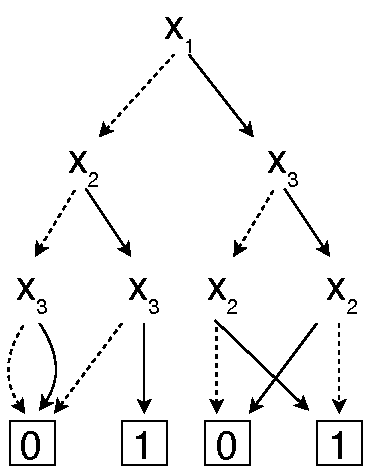
\includegraphics{figures/bdd1.pdf}}
    \subcaptionbox{\label{fig:ROBDD}ROBDD}
        {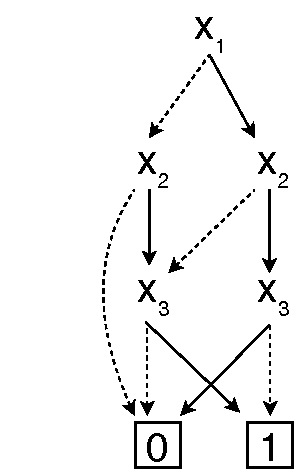
\includegraphics{figures/bdd2.pdf}}
    \caption{An example of BDD and ROBDD that represent the same BF $(\neg x_1 \land x_2 \land x_3) \lor (x_1 \land \neg (x_1 \lequal x_2))$}
    \label{fig:my_label}
\end{figure}

\begin{example}
\label{ex:BDD}
Figure~\ref{fig:BDD} shows an example of a BDD where edges to low children are dashed and to high children are full, non-terminal nodes are denoted by the variable they represent and terminal nodes are shown as boxes with the constant they represent. %We also show two copies of terminal nodes, this is only for better visualization, they are still the same two. To show nicer picture, the non-terminal nodes (boxe) 
This BDD represents the BF $(\neg x_1 \land x_2 \land x_3) \lor (x_1 \land \neg (x_1 \lequal x_2))$. 
\end{example}

To have simpler algorithms for BDDs, we actually use \emph{reduced ordered BDDs} (ROBDDs) which are BDDs such that 
\begin{enumerate}
    \item the variables on each path from the root of BDD to a terminal node are in the same order (possibly some of them are missing),
    \item the isomorphic (''the same looking'') subtrees are merged and
    \item nodes whose both edges go to the same subtree are deleted.
\end{enumerate}
They have the nice property that for a given variable order, each BF is represented by exactly one ROBDD. In the following chapters, when we use BDD we mean ROBDD.

\begin{example}
\label{ex:ROBDD}
Figure~\ref{fig:ROBDD} shows a ROBDD which represents the same BF as the BDD from Example~\ref{ex:BDD}. While the BDD from Figure~\ref{fig:BDD} does not have ordered variables the ROBDD always goes from root to terminal node with $x_1$ followed by $x_2$ and $x_3$. Also, one $x_3$ node was deleted because both edges coming from it ended in $0$. Furthermore, both $x_2$ nodes share an isomorphic subtree.
\end{example}

%To have simpler algorithms for BDDs, we usually want to have some ordering on the set of variables $V$ such that for each path from the root of BDD to the terminal of the BDD has nodes in this order. These BDDs are called ordered BDDs (OBDDs). The ordering of BDDs is important, because two BDD representations of the same BF in different orderings can have very different sizes. odkazat sa na obrazok ze tam je ordered 

%Two OBDDs with the same ordering representing the same BF can still be different, that is why we will actually work with reduced OBDDs (ROBDDs) which is an OBDD that merges isomorphic (''the same looking'') subtrees and deletes nodes whose both edges go to the same subtree. 

%As a final step 

% chceme mat linearne operacie ---> treba aby boli usporiadane ---> shannon expansion ---> ukazat operacie???
%When we have two BDDs, we want to have an effective way to compute their conjunction/disjunction. Such an algorithm should just traverse the BDDs in the same way while comparing the variables in the nodes. However, variables in the nodes on the paths from the root in general BDDs can occur in any order, which would cause problems with simple traversal of BDDs. To solve this we add an ordering on the set of variables $V$. The nodes in the BDD are then sorted based on this ordering. The resulting BDD is called an ordered binary decision diagram (OBDD).

%\begin{example}
%ukazat asi z previous example 2 orderings a povedat daco o tom ze operacie sa daju teraz implementovat jednoducho len prechadzanim stromom
%\end{example}

%nieco o ROBDD, ze pre kazde BF existuje prave jedno unikatne pre kazde zoradenie + ze vyber zoradenia je dolezity + ze da sa dynamicky preukladat???
%OBDDs still suffer from one problem -- for each BF we would like to have for given order on $V$ only one OBDD representing it. This is not the case, notice OBDDs on fig. ????? and ???. Both represents BF ??? but they are different. That is why we introduce reduced OBDDs (ROBDD) (vysvetlit lepsie ze to neni moj prinos). ROBDD is an OBDD such that all isomorphic sub-BDDs are merged and the nodes that have the same BDD as children are removed.

%\begin{example}
%porovnat nejake OBDD s jeho ROBDD, detailne (kde sa ukaze )
%\end{example}

For each operation on BFs (${\land}$, ${\lor}$, ${\neg}$), there is an algorithm on BDDs which can get the resulting BDD representing the application of the operation. For example, if we have a BDD representing BF $\psi_1$, we can get a BDD representing $\neg \psi_1$ by swapping terminal nodes $0$ and $1$. See for example Andersen~\cite{BDDdetails} for more details. %If we have another BDD representing BF $\phi_2$, we can get $\psi_1 \land \psi_2$ by using this algorithm.  Similarly an algorithm for ${\lor}$ can be defined.

%In the following we will use the term BDD instead of ROBDD.

%\section{And-Inverter Graphs - je ich treba rozobrat???}

\section{Quantifier Trees}
we talk shit about quantifier trees in this sectuibsddshuhusdf

\begin{definition}
  
\end{definition}

\chapter{State of the Art}
%problem - vytvorit algoritmus ktory zisti ze ci dana DQBF formula je splnitelna alebo nie pomocou BDDcok alebo jej podobnym strukturam (mozno dat do teorie)

%popisat tu aj nejak historiu DQBF, akoze napriklad ten clanok s henkins qunatifiers abo daco???

%Having laid out all the necessary theory we can now define the problem we are trying to solve and current implementations solving it.

%\section{The Problem of Satisfiability}
%Let $\psi$ be DQBF. The problem we are trying to solve is to tell whether this formula is satisfiable, that is if there exists model in which it is true. For BF, this problem belongs to NP-complete class of problems cite. If we move to QBF, the problem gets harder and belongs to PSPACE-complete class. As was shown in CITE, this problem for DQBF belongs in NEXPTIME-complete class of problems, that is it is even harder.

%\section{State of the Art}
%ake solvre existuju (vybrat tie s ktorymi budem porovnavat?), trocha viac popisat HQS a ze ako funguje aj HQSpre (lebo ho pouzivam) - ale fakt len zopar veci spomenut, mozno aj to ze mozme pouzit vytvaranie log. gates pretoze to menim do BDD ako to robia v HQS
In this chapter we give an overview of existing solutions and solvers which tackle the satisfiability problem of DQBF. Thereare already multiple surveys about DQBF~\cite{DQBFStateOfArtTalk,DQBFStateOfArt,DQBFStateOfArtNew}, we give only a short overview of most solvers and techniques. % that is why we just give a short updated overview here %(short for DQDPLL, iDQ, iProver and dCAQE). 
%However 
However, we go into more details for solver HQS, because it is currently the best performing solver (winner of the DQBF track of QBF Evaluation 2018~\cite{QBFeval18} and 2019~\cite{QBFeval19}) and the methods we use for developing our solver are based on the workings of this solver.
%current solutions, that already exist

%nieco o tom ze vacsina funguje na CNF, ale HQS a moje bude na NNF

%fast DQBF refutation - ze premienaju na QBF abo daco (bunsat)

\section{First Solution - DQDPLL}
The first solver that tackled the satisfiability problem for DQBF was based on DPLL~\cite{DPLL} algorithm which is successfully used for BF and QBF solvers. This algorithm works on formulas in CNF by searching for a satisfying assignment based on the clauses in CNF. By recursively choosing an assignment for literals and checking whether the remaining formula in CNF contains an empty clause (which implies unsatisfiability), DPLL searches trough all assignments until a satisfying one is found or all of them are decided to be unsatisfying. An adaptation called DQDPLL~\cite{DPLLalgorithm} was introduced for DQBF (in PCNF) which extended existing solutions for QBF by adding so-called Skolem clauses which encode the dependencies between existential and universal variables. However, by doing so the algorithm becomes too slow and results in an uncompetitive solver.

\section{Instantiation -- iDQ and iProver}
The first efficient DQBF solver, called iDQ~\cite{iDQandDQDIMACS}, is based on an instantiation technique used for solving Effectively Propositional Logic (EPR)~\cite{iProver}. This solver also works only on formulas in PCNF where in each step of the algorithm it tries to create a BF $\phi$ that is an overapproximation of an input DQBF. This is done by instantiating some set of clauses, that is it applies universal expansion locally to them. This BF $\phi$ is then checked for satisfiability, where if $\phi$ is unsatisfiable then the input DQBF is also not satisfiable, while if it is satisfiable, it must be checked if the resulting valuation is valid for the input DQBF. If it is not, then it is used to create more clause instances which are then used to refine this overapproximation.

Furthermore, a solver for EPR can also be used directly for DQBF. Because EPR belongs to the same complexity class as DQBF, there exists a polynomial-time reduction from DQBF to EPR~\cite{iDQandDQDIMACS}. This is used by EPR solver iProver~\cite{iProver} which transforms a DQBF in PCNF to an EPR instance and then solves this. %The results from QBF Evaluation 2018~\cite{QBFeval18} shows that iProver is more efficient than iDQ.  %In the SAT competition??? it turned out that iProver is more powerful compared to iDQ??

\section{Clausal Abstraction -- dCAQE}
Another DQBF solver called dCAQE~\cite{dCAQE} is based on clausal abstraction~\cite{ClausalAbstr}. This solver --- working again on DQBF in PCNF --- first puts universally and existentially quantified variables to some sets (called nodes) which are then divided into levels based on the ordering of dependencies of existential variables. The algorithm then constructs for each node on each level a BF that represents which clauses in CNF it can satisfy (for existential node) or falsify (for universal node). The algorithm then builds a candidate valuation by processing each level. For each level either this valuation is extended, or there is some conflict which means that the algorithm has to backtrack to some lower level and refine the abstraction, or the candidate valuation is a satisfying one which ends the algorithm.

%mozno spomenut fork splitting or something like that, v arXiv rozsirenej verzii maju nieco o tom v appendixe

\section{Quantifier Elimination -- HQS}
The next solver is based on quantifier elimination. This solver's basic premise is simple --- it iteratively chooses some universal variable for universal expansion (Theorem~\ref{thrm:unExpan}) thus eliminating it and then eliminates all existential quantifiers that are dependent on all leftover universal quantifiers using Theroem~\ref{thrm:exElim}.

\begin{algorithm}
\caption{Quantifier elimination algorithm}
\label{alg:QE}
\begin{algorithmic}[1]
\Function{SolveDQBF}{DQBF $\psi$ in PCNF}
\While{$V_{\psi}^{\forall}$ is not empty}%there is some universal variable $x$ in $\psi$
    \State choose $x$ from $V_{\psi}^{\forall}$
    \State $\psi = \forall\text{-expansion}(x,\psi)$% universal expansion
    \ForAll{$y \in V_{\psi}^{\exists}$ s. t. $D_y = V_{\psi}^{\forall}$} %existential variables $y$ such that they depend on all universal variables in $\psi$
        \State $\psi = \exists\text{-elimination}(y,\psi)$% existential expansion
    \EndFor
\EndWhile
\If{resulting BF $\psi$ is SAT}
	\State \Return SAT
\Else
	\State \Return UNSAT
\EndIf
\EndFunction
\end{algorithmic}
\end{algorithm}

Gitina et al.~\cite{HQSsimpleAlg} introduced the basic algorithm for solving DQBF in PCNF in this way. %(mozno spomenut ze to vlastne vymysleli aj v iDQ clanku, ako nejaky base solver ktory pouziva BDDcka) 
Algorithm~\ref{alg:QE} shows simple pseudocode of this. In every step, this algorithm chooses (using some heuristic) an universal variable to eliminate. The authors used a heuristic where the universal variable is chosen based on the number of existential ones that depend on it --- they choose the one that has minimal number of dependencies. After that, all the existential variables that depend on everything are also eliminated. To use this algorithm it is important to choose a good representation of the matrix of the DQBF. For this the authors chose and-inverter graphs~\cite{FRAIGs}. % (AIG) which are tree-like structures where non-terminal nodes represent conjunction, terminal nodes are variables and these are connected with two types of nodes: normal ones and those that represent negation. With a proper implementation of operations they can be optimised in such a way that they reuse parts of the graphs resulting in functionally reduced AIGs~\cite{FRAIGs}.

Following this technique, solver HQS was introduced~\cite{HQSquantifierElimination} which was enhanced by using QBF solver as a subprocedure. They still eliminate quantifiers in similar fashion but now they do it until the formula can be transformed to QBF (that is the dependency sets are linearly ordered). On this QBF they then run already existing solver for QBF called AIGSolve~\cite{AIGSolve} which can use more effective techniques developed for QBFs. Universal quantifiers to eliminate are chosen in the beginning in such a way that the number of universal eliminations is as small as possible while still the resulting formula is QBF. For this they build a dependency graph in which nodes are existential variables where $y_i$ is connected to $y_j$ if for their dependency sets it hold that $D_{y_i} \not\subseteq D_{y_j}$. They noticed that if this graph is acyclic, the formula can be seen as QBF. Furthermore, there is a cycle in this graph iff there is a simple cycle (between two nodes) in the graph. They use this to create an instance of MaxSAT problem which is a problem of finding a valuation of one BF while maximizing another formula. This instance then encodes which universal variables have to be eliminated so the dependency graph becomes acyclic while minimising the number of universal variables to eliminate. After finding the set of variables to eliminate, they follow with an improved quantifier elimination algorithm. They also improved it by adding a preprocessing step (see Section~\ref{sec:preprocessing}) and elimination of special types of variables called unit and pure. 

The algorithm was changed a bit again by Wimmer et al.~\cite{HQSdependencyElimination}. The authors were interested in whether it is possible to somehow remove specific dependencies from the list of dependencies of existential variable. They have shown that it is possible, albeit at the expense of adding a new existential variable. This is similar to the universal expansion (Theroem~\ref{thrm:unExpan}), but by removing just one dependency we add just one new existential variable. Let for example
\[\psi = \forall x_1 \dots \forall x_n \exists y_1(D_{y_1}) \dots \exists y_m(D_{y_m}) \itholds \phi\]
be a prenex DQBF where $\phi$ is a BF and $x_1 \in D_{y_1}$. We can now remove $x_1$ from $D_{y_1}$ by adding a copy of $y_1$ resulting in an equisatisfiable DQBF
\begin{multline*}
\forall x_1 \dots \forall x_n \exists y_1^0(D_{y_1} \setminus \{x_1\}) \exists y_1^1(D_{y_1} \setminus \{x_1\}) \exists y_2(D_{y_2})\dots \exists y_m(D_{y_m}) \\
\phi\left[((\neg x_1 \land y_1^0) \lor (x_1 \land y_1^1))/y_1\right].
\end{multline*}
Using this the authors do not look for a set of universal variables to eliminate, but for partial dependencies whose removal will result in a DQBF which can be transformed into QBF. Again, they create a dependency graph which is acyclic iff DQBF can be seen as QBF. But now they create a bipartite graph whose two sets of nodes are the set of universal variables and the set of existential variables which are connected based on whether universal variable is in the dependency set of existential one. Similarly to previous, they use this graph to solve an optimization problem that encodes which dependencies to remove to get QBF which can then be solved with AIGSolve.

Last but not least, Ge-Ernst et al.~\cite{HQSquantifierLocalization} have given a theoretical foundations for non-prenex DQBFs and the possibility to push and eliminate quantifiers inside formulas as explained in Section~\ref{sec:quantLocalization}. Using this they improve HQS by adding another step in the algorithm, where they first push quantifiers as much as possible into the formula, eliminate the existential variables using Theorem~\ref{thrm:exElim} and then return the formula back to the prenex form. After this they start with the elimination of universal quantifiers as was explained in previous paragraphs.

\section{Preprocessing}
\label{sec:preprocessing}
In previous sections, we give an overview of techniques used for implementations of different solvers. This sections explains some techniques that are used before the actual solvers run, called fittingly preprocessing.

\subsection{HQSpre}
The first and only preprocessing engine for DQBF called HQSpre~\cite{HQSpre1,HQSpre2,HQSpreJournal} took many techniques used for QBF preprocessing and lifted them to the DQBF case. We explain only one technique here, called \emph{gate extraction}. As was mentioned in Section~\ref{sec:BF:CNF}, transforming BF to an equisatisfiable formula in CNF can result in polynomial increase of the size of the formula by adding new variables. Gate extraction works in opposite direction --- it tries to extract this newly introduced variables and turn the formula back into one that is not in CNF. This does not mean that gate extraction works only on formulas in CNF, it can be used generally by finding connections between variables which make it possible to replace a variable by some Boolean function of existing variables. However, this technique can only be used by solvers which can work on DQBFs which are not in PCNF. Currently, that is only HQS. For a thorough explanation of other techniques used by HQSpre we refer the reader to the work by Wimmer et al.~\cite{HQSpreJournal}. 

\subsection{Approximations}
Another technique which is used in some solvers as preprocessing step is to find some BF or QBF approximations which can be used with existing solvers for BFs/QBFs to potentially give us faster result about the input DQBF (satisfiability for underapproximations, unsatisfiability for overapproximations). Gitina et al.~\cite{HQSsimpleAlg} introduced QBF approximations which are created by changing the dependencies of existential variables that result in QBF with the same matrix. However, these approximations can be precise only up to some level. By adding some information to these QBF overapproximation (thus changing the matrix), Finkenbeiner et al.~\cite{FastDQBFRefutation} were able to create more and more precise QBF overapproximations. For more thorough explanation of these approximations see again the work by Wimmer et al.~\cite[Section~3]{HQSpreJournal}.

\subsection{$\PSPACE$ subclass}
The last preprocessing technique is simply put just a check whether DQBF does not belong to a subclass of problems which are in $\PSPACE$ and if it does, it is transformed to QBF (which is $\PSPACE$-complete) on which existing QBF solver is run. The simplest such subclass would be those DQBFs whose dependencies are linearly ordered. Then it can be easily transformed into QBF by reordering the quantifiers. Scholl et al.~\cite{PSPACEsubclass} investigated whether there is some another DQBF subclass which is in $\PSPACE$. They show that DQBFs where the dependency sets are either equal or pairwise disjoint can be transformed into QBFs with just linear increase in size. Thus having a check on whether an input DQBF belongs to this class before running a DQBF solver and if it does transforming it into QBF and running a QBF solver can improve the efficiency. They show this by adding this preprocessing step to HQS which results in increase of solved instances.

%As a note toto vzislo z toho, ze clanok zrobil dajaky system ktory je rozsirenie QBF systemu kde pridali fork extension pravidlo. They showed that this system is complete and sound for DQBF, however, in dCAQEclanok (ale v appendixe extended version) and PSPACEclanok ukazali ze to tak nie je (nie je complete ci co). Obe tieto clanky ukazali ze tento system je complete pre tuto PSPACE classu. Zaroven dCAQE vyuziva tento fork extension ???a zle si myslia ze tato classa je NEXPTIME??? vo svojom algoritme, takze je moznost ze ich algoritmus nefunguje pre celu classu DQBF

\chapter{Our Algorithm}
\label{chap:algorithm}
%TODO: decide the name, our/suggested/new/... algorithm

In this chaoter we introdice our algorithm for solving satisfiability of DQBF using BDDs. First we give a high level eplanation of the algorithm and then we explain each part of it showing different heuristics for solving it???

\section{High level defintion???}
\begin{algorithm}
\caption{???}
\label{alg:????}
\begin{algorithmic}
\Function{SolveDQBF}{quantifier tree ???with root $r$??? ???}
\State \Call{Localise}{???}
\State (prefix, $\phi$) = \Call{TurnToBDD??}{???}
\State \Call{ElimAllUnivVars}{DQBFprefix, $\phi$}
\If{$\phi = 0$}
    \State \Return UNSAT
\Else
    \State \Return SAT
\EndIf
\EndFunction
\end{algorithmic}
\end{algorithm}
The algorithm is shown in .... is a high level definition of out algorithm. In the next sections we explain more thoroughly each part of the algorithm. It takes as an input a DQBF $\psi$ in NNF represented using quantifier tree. First, using some heuristic function localise(????) recursively pushes the quantifiers inside the formula, usually by using rules from Theorem~\ref{thrm:quantLocalEq}. Next, we transform this quantifier tree into a tuple of quantifier prefix and a BF represented by BDD by recursively turning children of each node into this tuple of prefix and BDD and combining them together. something about pulling the quantifiers back??? the quantifiers are pulled back, however, we remove some of them??? During this some quantifiers can be eliminated by using theorems for quantifier eliminations (Theorem~\ref{thrm:unExpan} and \ref{thrm:exElim}), Section??? shows different heuristics how to decide which quantifiers are eliminated. Finally, the leftover quantifiers in the prefix are eliminated resulting in BDD which represents either $0$ or $1$ which tells us whether the formula is satisfiable or not.

vysvetlit co je to quantifier tree (proste reprezentacia DQBF, kde kazdy non terminal node reprezentuje operaciu and alebo or na children (co su subformule) a pri kazdom tomto node su ulozene kvantifikatory; terminal nodes su literals) -- hodit mozno do kapitoly 1, plus obrazok

algoritmus zacina s tymto stromom kde vsetky kvantifikatory su v root, pomocou theoremu o lokalizacii ich strcime dnu (popisat heuristiku ze ako ich strkame), potom rekurzivne prechadza tento strom, kde ziska s children formule, z ktorych vytiahne kvantifikatory a maticu prevedie do BDD a potom nejakou heuristikou sa rozhodne ktore kvantifikatory sa odstrania, tie sa odstrania (pouzitim theorems o odstranovani - pridat mazanie ak nie je v support set, nejakou heuristikou sa rozhodne v akom poradi) a return zvysny prefix s maticou v BDD


\section{Heuristic to how to localise variables/Implementation???? of localise(??)}
\begin{itemize}
    \item we do not localise - for simple solver
    \item when we localise for conjuction and univ/exist quantifier we choose this and this children to put it in etc. for disjunction and univ/exist this and this etc.
\end{itemize}

\section{Heuristics of deciding what to do on each level of quantifier tree}
\begin{itemize}
    \item nothing - simple solver (maybe have it a heuristic which variables to localise???, so we say none and we get simple solver; we could put it with how to localise???)
    \item remove everything possible (all universal vars and possible exist. vars, in iteration -> one universal var, all possible existential vars (based on theorem~\ref{thrm:exElim}) and so on) - tree solver
    \item remove only exist vars (or maybe just some univ. vars - those that only few exist vars depend on or those that will allow me to remove some exist vars)???
    \item remove some dependencies to be able to remove exist vars???? - not possible??
\end{itemize}


\section{Heuristics for order of elimination of universal variables}
\begin{itemize}
    \item the order is set on the beginning based on the number of existential variables that depend on them (from lowest to highest), so the created duplicates do not count in, i.e. for \[\forall x_1 \forall x_2 \forall x_3 \exists y_1(x_1, x_2) \exists y_2(x_1,x_2) \exists y_3(x_3) \exists y_4(x_3) \exists y_5 (x_3),\] the order is $x_1, x_2, x_3$, because both $x_1$ and $x_2$ only two depend on them, for $x_3$ it is three
    \item similarly, but the next universal variable to eliminate is the one with the minimal number of existential variables that depend on them (so also the existential duplicated count here), i. e. for the previous example, first $x_1$ is removed, but then we have \[\forall x_2 \forall x_3 \exists y_1(x_2) \exists y_2(x_2) \exists y_1'(x_2) \exists y_2'(x_2) \exists y_3(x_3) \exists y_4(x_3) \exists y_5 (x_3)\] and so $x_3$ is removed next, because there are four ex. variables (two original, two duplicates) that depend on $x_2$ now
    \item something with creating depency tree, to find existential variables to remove as fast as possible (not sure if possible) --- maybe possible, basically remove those universal vars that will make it possible to remove as much existential vars as possible on the level??? 
\end{itemize}

\chapter{Implementation}

\chapter{Experimental results}
popisat na com testujeme a ze sme pouzili benchexec

povedat ze sme najprv pustili HQSpre (odkaz na sekciu a asi aj znova citovat) bez gate detection, odfiltrovali sme results ktore boli vyriesene HQSpre alebo uz HQSpre prekrocil limity... vysledok tohto sme hodili do iDQ, iProver, dCAQE

pre HQS a moj pouzivame -> ak gate detection zisti ze mame viac ako n gates (v HQS maju teraz 5) tak pustime znova HQSpre ale teraz uz aj s tym ze chranime tieto gates aby sme ich potom mohli pouzit

cas HQSpre bez gate detection zaratavame do vsetkych solvrov, tym silmulujeme to co robi HQSnp???

benchmarks:
\begin{itemize}
    \item PEC - vid \cite{HQSquantifierLocalization} ze co vsetko citovat, su to asi folders Finkbenier, Scholl a Biere v z tej stranky stiahnute co je tam odkaz v tom istom clanku
    \item controller synthesis problems - to iste, folder je ale iba Bloem
    \item ziskane zo SAT - to iste, folder je ale iba Balabanov
    \item BoSy - vid \cite{dCAQE}, nie su ale zverejnene, skusit asi popytat
\end{itemize}
Zrobit asi pre kazdy tento benchmark sekciu a porovnat - grafy, tabulky atd, neviem este. Potom zrobit velky graf kde dam vsetko dohromady mozno, nech vidno spolu ze ake to je. A mozno dat z QBFeval'19, ze povedat ze je to suhrn vybratych benchmarks z tychto (okrem asi BoSy), tak aby nijaky nedominoval a nejak su pekne rozdelene ci co a ukazat na tom ????

Este mozno budem porovnavat navzajom rozne heuristiky pouzite v mojom a potom budem porovnavat najlepsiu???? s ostatnymi????

\chapter{Conclusion}


\begingroup
\setlength{\emergencystretch}{8em}
\printbibliography[heading=bibintoc]
\endgroup

%\chapter{Inserting the index}
%After using the \verb"\makeindex" macro and loading the
%\texttt{makeidx} package that provides additional indexing
%commands, index entries can be created by issuing the \verb"\index"
%command. \index{dummy text|(}It is possible to create ranged index
%entries, which will encompass a span of text.\index{dummy text|)}
%To insert complex typographic material -- such as $\alpha$
%\index{alpha@$\alpha$} or \TeX{} \index{TeX@\TeX} --
%into the index, you need to specify a text string, which will
%determine how the entry will be sorted. It is also possible to
%create hierarchal entries. \index{vehicles!trucks}
%\index{vehicles!speed cars}

%index:
%  \makeatletter\thesis@blocks@clear\makeatother
%  \phantomsection %% Print the index and insert it into the
%  \addcontentsline{toc}{chapter}{\indexname} %% table of contents.
%  \printindex

\appendix %% Start the appendices.
\chapter{An appendix}
Here you can insert the appendices of your thesis.

\end{document}
